\section{Results from the Pilot Deployment}
\label{sec:pilot-study}

To evaluate the capabilities of the OPQ Sensor Network, 15 OPQ Boxes were deployed at the University of Hawaii Manoa campus over the course of three months in the Fall of 2019.  The University of Hawaii campus is an isolated microgrid connected to the Oahu powergrid only via a single 46kV feeder. The UH Campus also has traditional, revenue-grade electrical meters deployed across various levels of the power delivery infrastructure. While the primary purpose of these meters is to monitor power consumption, they do include power quality monitoring capabilities. Data from these meters were used as ground truth for validation studies of the OPQ sensor network.

The University of Hawaii power grid is interesting in that it supplies a highly diverse infrastructure. Beyond traditional residential equipment such as computers and consumer grade electronics, the UH power grid powers scientific and laboratory equipment, machine shops, and server farms. All of these elements have varying requirements/tolerances for power quality anomalies as well as different levels of power quality “pollution”. Furthermore, some of the electricity consumers in the UH campus are entirely unique. For example, the free electron laser located in the Watanabe Hall is one of only ten in the world, and the impact/sensitivity of power quality on the instrument are completely unstudied.

The pilot study had the following major goals:

\begin{enumerate}

\item {\em Evaluation of sensor data accuracy and quality.} While we conducted extensive laboratory tests of the sensor network, the pilot study enabled us to evaluate the accuracy and utility of our hardware devices and power quality data collection procedures in a real-world setting. Does an OPQ sensor network measure power quality (and detect anomalies) as well or better than conventional building-level electrical meters?

\item {\em Evaluation of the triggering system.} The OPQ Makai triggering system provides a novel two-way communication between sensors and the cloud, resulting in a triggering system with unique capabilities.  Does the triggering system provide efficiencies not available from more conventional approaches? Does it provide data enabling analysis opportunities not available through more conventional approaches?

\item {\em Evaluation of the information architecture.} OPQ Mauka implements a tiered, hierarchical information architecture.  The pilot study enabled us to evaluate this information architecture.  Would this information architecture prove useful with real world data? Could actionable insights emerge from low-level sensor data?

\item {\em Evaluation of cloud data storage management.} OPQ Mauka manages data storage through a "time to live" (TTL) mechanism, which results in data being discarded if it is not found to be useful and thus "promoted" to a higher level of the information hierarchy within a defined period of time.  The pilot study enables us to evaluate this approach. Does this mechanism allow sensor network designers to determine upper bounds on storage requirements? Is information thrown away prematurely because it was not found to be useful within the time limits?

\end{enumerate}

\subsection{Descriptive statistics}

\begin{tcolorbox}[colback=red!5!white,colframe=red!75!black,title=ANTHONY]

Could you provide descriptive statistics for this section? This includes the start and end dates of the pilot study, the total number of data elements collected at each level of the information hierarchy, and for incidents and phenomena, the total number of each type of incident and event. Perhaps the size of the database?
\end{tcolorbox}


\subsection{OPQ Boxes provide valid and reliable collection of power quality data}

The first goal of the pilot study was to assess how well an OPQ sensor network is able to collect basic power quality data. To do this, we compared data on voltage and frequency collected by OPQ Boxes with data on voltage and frequency collected by the revenue-grade building level power monitors.  The results are shown in Figure \ref{fig:opqbox-f-v-validation}.

\begin{figure}[ht]
	\centering
	\begin{subfigure}{.5\textwidth}
	  \centering
	  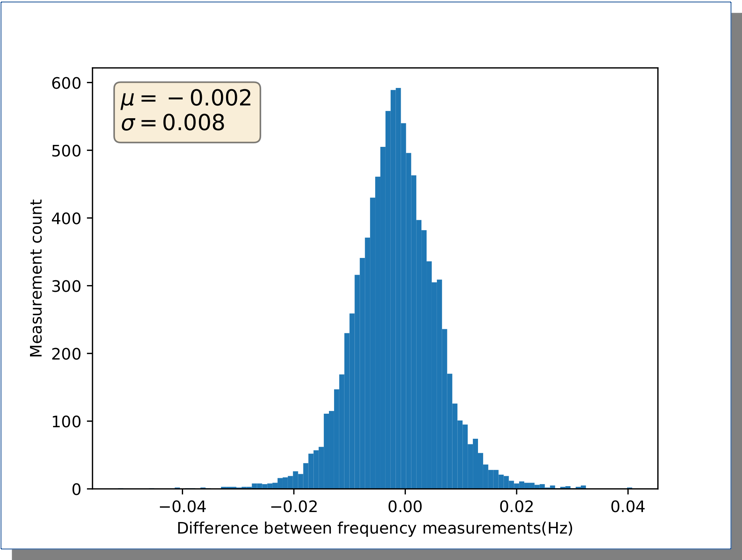
\includegraphics[width=0.9\linewidth]{images/pilot/opqbox-frequency-validation.png}
	  \caption{Frequency differences}
	  \label{fig:opqbox-validation-1}
	\end{subfigure}%
	\begin{subfigure}{.5\textwidth}
	  \centering
	  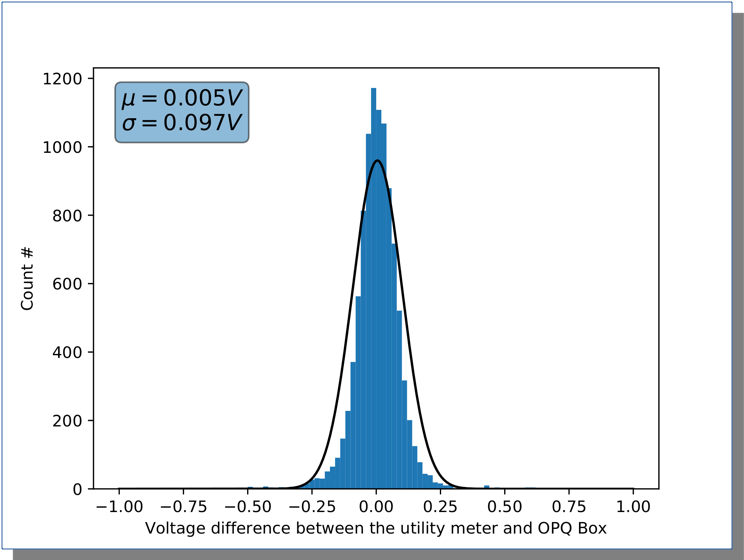
\includegraphics[width=0.9\linewidth]{images/pilot/opqbox-voltage-validation.png}
	  \caption{Voltage differences}
	  \label{fig:opqbox-validation-2}
	\end{subfigure}
	\caption{Validation of (a) Frequency and (b) Voltage}
	\label{fig:opqbox-f-v-validation}
\end{figure}

As the charts illustrate, there is very little difference between the frequency and voltage values collected by OPQ Boxes and the building meters.

Validating THD and transient data, the other two basic power quality measures collected by OPQ Boxes, was more challenging.

Figure \ref{fig:opqbox-thd-validation} shows the results of comparing values of THD collected by OPQ Boxes and building meters.

\begin{figure}[ht]
  \centering
	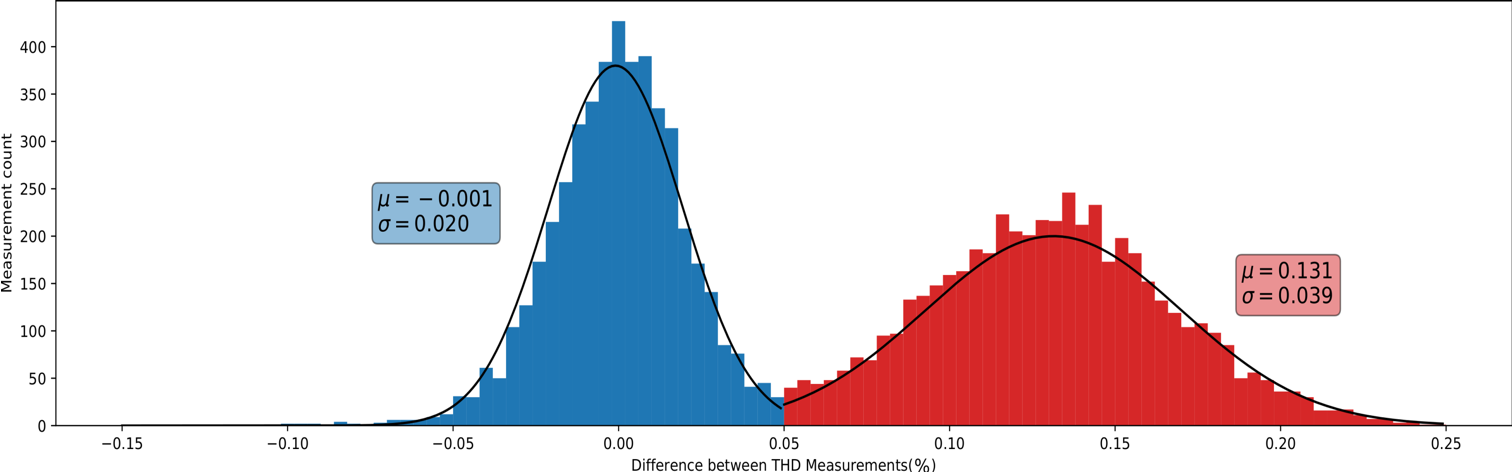
\includegraphics[width=0.8\linewidth]{images/pilot/opqbox-thd-validation.png}
	\caption{THD differences}
	\label{fig:opqbox-thd-validation}
\end{figure}

Unlike frequency and voltage, where there was very close alignment between OPQ Boxes and building meters, THD data shows two peaks, one of which is indicates a kind of "offset" of approximately 0.13% by the OPQ Boxes from the building meters.

\begin{tcolorbox}[colback=blue!5!white,colframe=blue!75!black,title=SERGE]
Could you augment the above paragraph with a few sentences about why you think the THD validation looked like it did? I know you covered this in your defense but I forgot.
\end{tcolorbox}

Unfortunately, we unable to perform validation of transient data collection, because building meters did not provide us with access to that information.

\begin{tcolorbox}[colback=blue!5!white,colframe=blue!75!black,title=SERGE]
Could you add an additional sentence or two to the above paragraph about transient data validation? Maybe more about why we couldn't do it, or what the implications of non-validation might be?
\end{tcolorbox}

\subsection{OPQ Makai's triggering system provides advantages with respect to bandwidth and computation}

The pilot study provided an opportunity to collect data on the resources required by an OPQ sensor network with respect to cloud-level network resources and server-level computation overhead.

To assess network bandwidth utilization, we analyzed the data stream of frequency and voltage collected by OPQ Boxes, and the resulting network bandwidth utilized by the OPQ Makai triggering algorithm. Over the course of a typical day, OPQ Makai requested approximately 136 MB of data from the deployed OPQ Boxes.  We then calculated how much data would be sent by a power quality meter using more conventional triggering approach in which exceeding a threshold would automatically result in sending waveform data, and found that, under the same conditions, approximately 1025 MB would be sent to the cloud, or eight times the network bandwidth.

\begin{tcolorbox}[colback=blue!5!white,colframe=blue!75!black,title=SERGE]
Please review and improve the above paragraph.
\end{tcolorbox}

To assess computational cost, we again analyzed the data stream for a typical day...

\begin{tcolorbox}[colback=blue!5!white,colframe=blue!75!black,title=SERGE]
Please finish the above paragraph by describing in words the histogram in slide 38 of your thesis defense presentation, where you show that Napali uses much less computational resources.
\end{tcolorbox}

\subsection{The OPQ Information Architecture provides a means to produce actionable insights}

\subsection{The OPQ Information Architecture provides predictable upper bounds on storage resources}

\subsection{OPQ Mauka provides useful adaptive optimization capabilities}



